In this prospectus report, the potential impacts of DER (distributed energy resource) integration on the distribution network has been reviewed. Moreover, the challenges of coordinating the system voltage regulation and optimally managing system energy under a real-time pricing scheme have also been explored. The reviews lead to the identification of gaps in the current methods of voltage regulation and optimum energy management. Consequently, two algorithms were proposed that would help in the integration of DERs into the grid.

A coordinated voltage control algorithm based on the concepts of electrical distance calculation and voltage sensitivity analysis has been developed and presented. The algorithm proposed, has the ability to coordinate the reactive power reference points for the distributed generation and traditional voltage regulation devices located along the feeder, taking into account their potential impacts on the entire system. By using this approach, a reduction in the use of traditional regulation devices can be achieved and the voltage profiles along the network can be controlled for the most part by just using the already existing DG inverters present on the network. The planned additions to this work are as follows.

\begin{itemize}
    \item Develop a state estimation technique which can determine the system voltage angle from real and reactive power readings.
    \item Perform real-time validation of developed algorithm
\end{itemize}

Moreover, a novel energy management system aimed to determine the optimal operation of a single grid connected DS has been proposed. The management scheme is designed to optimize the charging and discharging of grid-connected energy storage by formulating the problem as a graph search and solving the graph search using the A* search algorithm. The A* based ESM is tested using real data collected from the SUNGRIN project, NYISO, and PG\&E. It also considers both a net metering scenario and a different sell back price scenario where the buying price of energy is different from the selling price.  The planned additions to this work are as follows.

\begin{itemize}
    \item develop an algorithm capable of dealing with multiple sources while maintaining system constraints.
    \item Perform real-time validation with multiple sources.
\end{itemize}

% \section{Current state of the work}
% In the current state the author has developed ...
%\section{Future Work Schedule}


\section{Publications}
\subsection{Accepted conference paper}
\begin{itemize}
    \item A. Newaz, J. Ospina and M. O. Faruque. Coordinated Voltage Control in Distribution Systems with Distributed Generations. [Accepted] \textit{IEEE PES General Meeting,2019}.
    \item Nikhil Gupta, Griffin Francis, Juan Ospina, Alvi Newaz, Emmanuel G Collins, Omar Faruque, Rick Meeker, Mario Harper. Cost Optimal Control of Microgrids Having Solar Power and Energy Storage. \textit{2018 IEEE/PES Transmission and Distribution Conference and Exposition (T\&D), 1-9}
    \item A Hariri, A Newaz, MO Faruque. A Matlab-openDSS hybrid simulation software for the analysis of PV impacts on distribution networks. \textit{2016, 59th Int. Soc. Autom. Power Ind. Division Symp., 1-12}
\end{itemize}

\subsection{Accepted Journal Paper}
\begin{itemize}
    \item MMS Khan, MO Faruque, A Newaz. Fuzzy logic based energy storage management system for MVDC power system of all electric ship. \textit{2017, IEEE Transactions on Energy Conversion 32 (2), 798-809.}
    \item A Hariri, A Newaz, MO Faruque. Open-source python-OpenDSS interface for hybrid simulation of PV impact studies. \textit{2017, IET Generation, Transmission \& Distribution 11 (12), 3125-3133.}
    \item J Ospina, A Newaz, MO Faruque. Forecasting of PV plant output using hybrid wavelet-based LSTM-DNN structure model. \textit{2019, IET Renewable Power Generation 13 (7), 1087-1095.}
\end{itemize}

\subsection{Submitted Journal Paper}
\begin{itemize}
    \item A. Newaz, J. Ospina and M. O. Faruaue. A Graph Search Based Optimal Control Technique for Enterprise Level Energy Storage Based on Forecasting of PV, Load and Real-Time price of Energy. [Submitted] \textit{IEEE transaction on industrial electronics.}

\end{itemize}

%\subsection{Paper under construction}
\subsection{Future Work and Schedule}
In the upcoming time, real-time validation of the coordinated voltage control algorithm will be performed and the results will be published. The graph search based energy management system will be updated to include multiple DERs and system constraints. A grantt chart for important milestones is shown in fig. \ref{fig:GANTT}.

\begin{figure}[!ht]
    \centering
    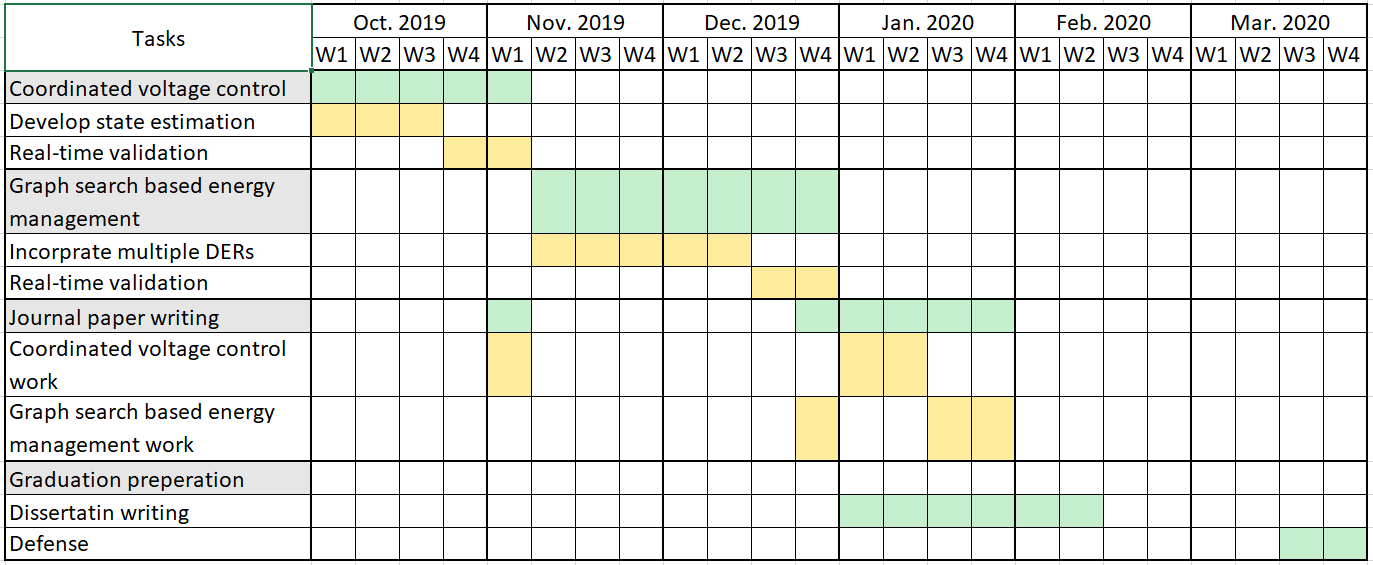
\includegraphics[width = \linewidth]{figs/Gantt2.png}
    \caption{Grantt chart for future tasks}
    \label{fig:GANTT}
\end{figure}
